\section{TEP-Net Model}
\label{sec:baselineModel}

In the literature rails are often detected without distinction between all rails visible in an image and the rail the train continues.
\cite{tepNet2024} therefore proposes a regression-based approach, which restricts the model to predict a single track.
The idea comes from various lane detection methods in autonomous driving applications for road cars and is fitted the rail domain.

Although rails can be represented by second or third-degree polynomials in curves \cite{PolyLaneNetRoad2021}, they may also take more complex geometric shapes.
Hence, limiting the output to presumed forms is discouraged.
Therefore, the method used in \cite{tepNet2024} employs spline interpolation to describe such complex structures.

\begin{figure}[H]
    \centering
    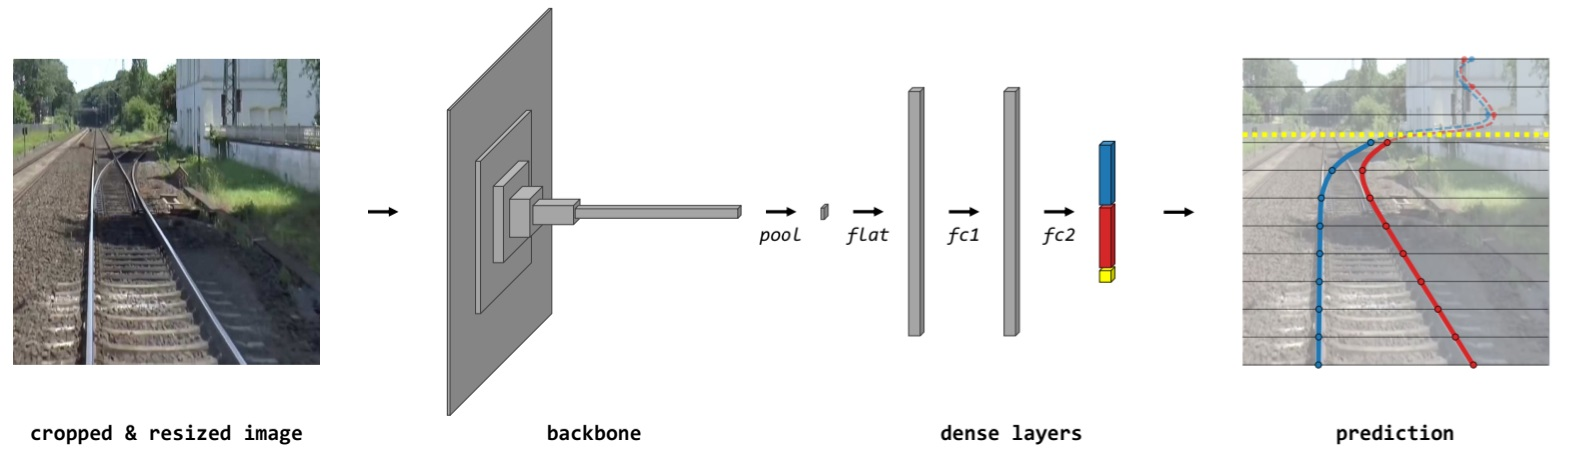
\includegraphics[width=\linewidth]{PICs/Baselinepaper/TEP-Net_model.jpg}
    \caption{\ac{TEP}-Net model architecture\cite{tepNet2024}. The input of the model is a cropped and resized image and the output of the model are the $x$-values for the left and right rail on each anchor line plus an additional value for the $y$-limit.}
    \label{fig:TEP-Net_model}
\end{figure}

As shown in the prediction of \autoref{fig:TEP-Net_model}, a set of horizontal lines are overlayed in the cropped image.
The number of $y$-lines or "anchors" is determined by a hyperparameter.
They are uniformly distributed along the $y$-axis. For each line, two $x$-values are predicted.
One for the left rail and one for the right rail.
The second and fourth images in the bottom row of \autoref{fig:tepNet_dataaugmentation} and the prediction image of \autoref{fig:TEP-Net_model} show that rails do not necessarily cross with anchor lines at the top of image crops.
Therefore, an additional $y$-limit is predicted, which gives information up to which anchor the rail should be detected.
Anchors and their $x$-values above this horizon line do not hold valuable information and are ignored.

For this novel regression task, a new model architecture is created.
For this model widely used backbone architectures like ResNet and EfficientNet are chosen.
These backbones extract relevant features from the cropped images reducing the spatial dimensions and increasing channel size to a high number.
After that, the feature map's number of channels is reduced to a predefined size with a 1x1 Conv2d layer \cite{pytorch_conv2d_docu} and flattened to a vector.
This feature vector serves as the input for the prediction head, which consists of two fully connected layers \cite{pytorch_linearLayer_docu} in series.
The size of the linear layers is set with a hyperparameter.
In the last layer, a reduction leads to the resulting prediction vector with the dimension $2 \times H + 1$.
$H$ is the number of anchors.
This vector includes the entire information of one prediction.
The first set of values with size $H$ is for the left rail, another $H$ set for the right rail and the $+ 1$ is for the last values being the horizon line.

This architecture's policy for value ranges does not restrict the $x$-values in any way.
This way predictions can be outside of a crop and the model can learn that sometimes the rails extend out of the viewed field.
The $y$-limit on the other hand is constrained to a range between 0 and 1 with a Sigmoid function.

The introduced model architecture can be classified as an end-to-end framework.
This means the model can be trained and used for inference without any steps in between.
It takes in raw data and results in a complete prediction.
